\documentclass[10pt,twocolumn]{article}
\usepackage[letterpaper,margin=0.75in]{geometry}
\usepackage{graphicx}
\usepackage[hidelinks]{hyperref}
\setlength{\columnsep}{0.25in}
\title{Geometry, Pose, and Descriptions for Social-Norm Reasoning}
\author{Idea 5: exploratory analysis draft for author review}
\date{October 4, 2026}
\begin{document}
\maketitle
\noindent\textbf{Review status.} This standalone preview presents a partial computational experiment, stopped at the user's request. Human review of predicted representations, captions, and the final interpretation is pending. Insert the accompanying section into the team's ICML report after reviewing it; this preview is not the complete team submission.
% Draft section for the existing ICML report; author review required.
\section{Analysis: Explicit Geometry, Pose, and Descriptions}
\paragraph{Questions and protocol.} We investigate whether RGB-derived pose, instance segmentation, and relative depth improve zero-shot social-norm decisions, separately and together, and whether textual descriptions change the effect. We retain the fixed 40 source-disjoint EgoNormia examples and five pre-action frames per clip (200 frames). We use frozen MediaPipe body/hand extractors, YOLOv8n-seg COCO instance masks, and Depth Anything V2 Small relative depth. Maps are derived visual representations, not independent sensor modalities; estimated depth is not measured distance. A local community 8-bit Qwen3-VL-32B-Instruct checkpoint selects an action and then a justification with greedy decoding and independently permuted options, fixed across conditions. No training is performed.
\paragraph{Descriptions and controls.} Each representation is tested with images alone and with attached descriptions. RGB descriptions are generated by Qwen from the RGB grid without answer options, labels, taxonomy, or dataset descriptions. Processed-image descriptions deterministically summarize the extractor outputs and their limits. Repeated RGB controls match one or three auxiliary slots at identical RGB resolution. Shuffled-all uses another source's three maps and associated descriptions. Text lengths are not matched, so image-only/description ablations are essential. This custom pilot is not an official leaderboard replication.
\paragraph{Results.} The table reports joint action-and-justification correctness; full action/justification results and raw responses are in the repository.
\begin{center}\small\setlength{\tabcolsep}{3pt}
\begin{tabular}{lrr}
Input & Images only & With descriptions \\
\hline
RGB & 3/35 & 2/35 \\
RGB + pose & 3/35 & 2/35 \\
RGB + segmentation & 4/35 & 2/35 \\
RGB + depth & 4/35 & 2/35 \\
RGB + all three & 4/35 & 3/35 \\
RGB + repeated RGB & 3/35 & 2/35 \\
RGB $\times$ 4 & 3/35 & 2/35 \\
RGB + all three shuffled & 5/35 & 2/35 \\
\end{tabular}\end{center}
The user stopped inference after 562 of 640 planned condition rows. All table entries use the same 35 clips completed under all 16 conditions. The 2 additional rows are preserved but excluded from this matched table. No further inference was performed.
With images alone, all three minus RGB joint accuracy is +2.9 percentage points; 1 items improve and 0 worsen. The paired 95\% bootstrap interval is [+0.0, +8.6]. With images and descriptions, all three minus RGB joint accuracy is +2.9 percentage points; 1 items improve and 0 worsen. The paired 95\% bootstrap interval is [+0.0, +8.6]. 
RGB alone is jointly correct on 3/35, compared with 4/35 for all-three images. Shuffled-all images reach 5/35, exceeding the aligned-map result. All-three with descriptions scores 3/35; therefore these observations do not establish a consistent advantage from aligned geometry or attached descriptions. The low absolute scores warrant review of the saved prompts and image evidence before interpreting the result as a model capability estimate. The matched cohort is the first fully processed prefix of the fixed ordering, not a subset selected for successful outcomes.
\paragraph{Illustrative cases.} In the climbing-equipment example (\texttt{54adfe07}), RGB and pose-only select the incorrect none option, while segmentation-only, depth-only, and all-three images select the correct equipment-check action and justification. Repeated RGB still fails, but shuffled auxiliary maps also succeed, and descriptions remove the gain. Thus this recovery does not isolate an effect of aligned geometry. In the shopping example (\texttt{e93fdf27}), all-three images with descriptions select the correct friend-opinion action and justification, while RGB, individual representations, repeated RGB, and shuffled-all fail. Maps alone also fail there; unmatched description lengths and the combined visual/text change prevent a geometry-only interpretation. These examples should be inspected alongside the complete paired counts, rather than selected as evidence of general improvement.
\paragraph{Extended agent failure diagnostics.} On the first 15 fixed-order RGB examples, the agent is jointly correct on 11/15. All 4 failures from the additional ten-case baseline were retested under the remaining 15 conditions. All-three images recover 1/4; all-three with descriptions recover 1/4. The cohort is selected by baseline errors, and the agent accumulates context, so these are recovery diagnostics rather than unbiased accuracy or causal geometry estimates. Complete controls and image evidence are in the accompanying failure gallery.
\paragraph{GPT agent feasibility pilot.} A spawned agent configured with the requested \texttt{gpt-5.6-sol} override viewed actual image grids and selected answers without gold labels on the first five examples. Its context accumulates across cases and conditions, so this is an agent-workflow feasibility check, not a clean stateless API comparison or model ranking. all descriptions: 5/5 joint-correct. depth descriptions: 5/5 joint-correct. pose descriptions: 5/5 joint-correct. rgb descriptions: 5/5 joint-correct. rgb images: 5/5 joint-correct. segmentation descriptions: 5/5 joint-correct. 

\paragraph{Discussion (author review required).} Inspect which gains, declines, and answer changes survive the repeated-image and shuffled-map controls before attributing them to aligned geometry. Gains introduced only by descriptions may reflect language scaffolding or caption errors rather than new visual information. Sparse pose output, COCO-limited masks, and uncalibrated depth each require qualitative review. This small frozen-model experiment does not test the proposal's fine-tuning, and the 32B run's new prompt prevents a clean size-only comparison with the earlier 8B pilot. EgoNormia labels were used for exploratory scoring, so it remains excluded from training but is not untouched. Preserve failed outputs and evaluate any future adaptation on independently reserved examples under matched budgets.
% AI DISCLOSURE: Codex designed and implemented this expanded experiment, generated summaries/figures and drafted this section. Qwen generated RGB captions and experimental predictions; MediaPipe, YOLO, and Depth Anything generated derived representations. A GPT-5.6-sol-configured agent made a blinded tool-using pilot. Human interpretation and review remain pending.

\begin{figure*}[t]
\centering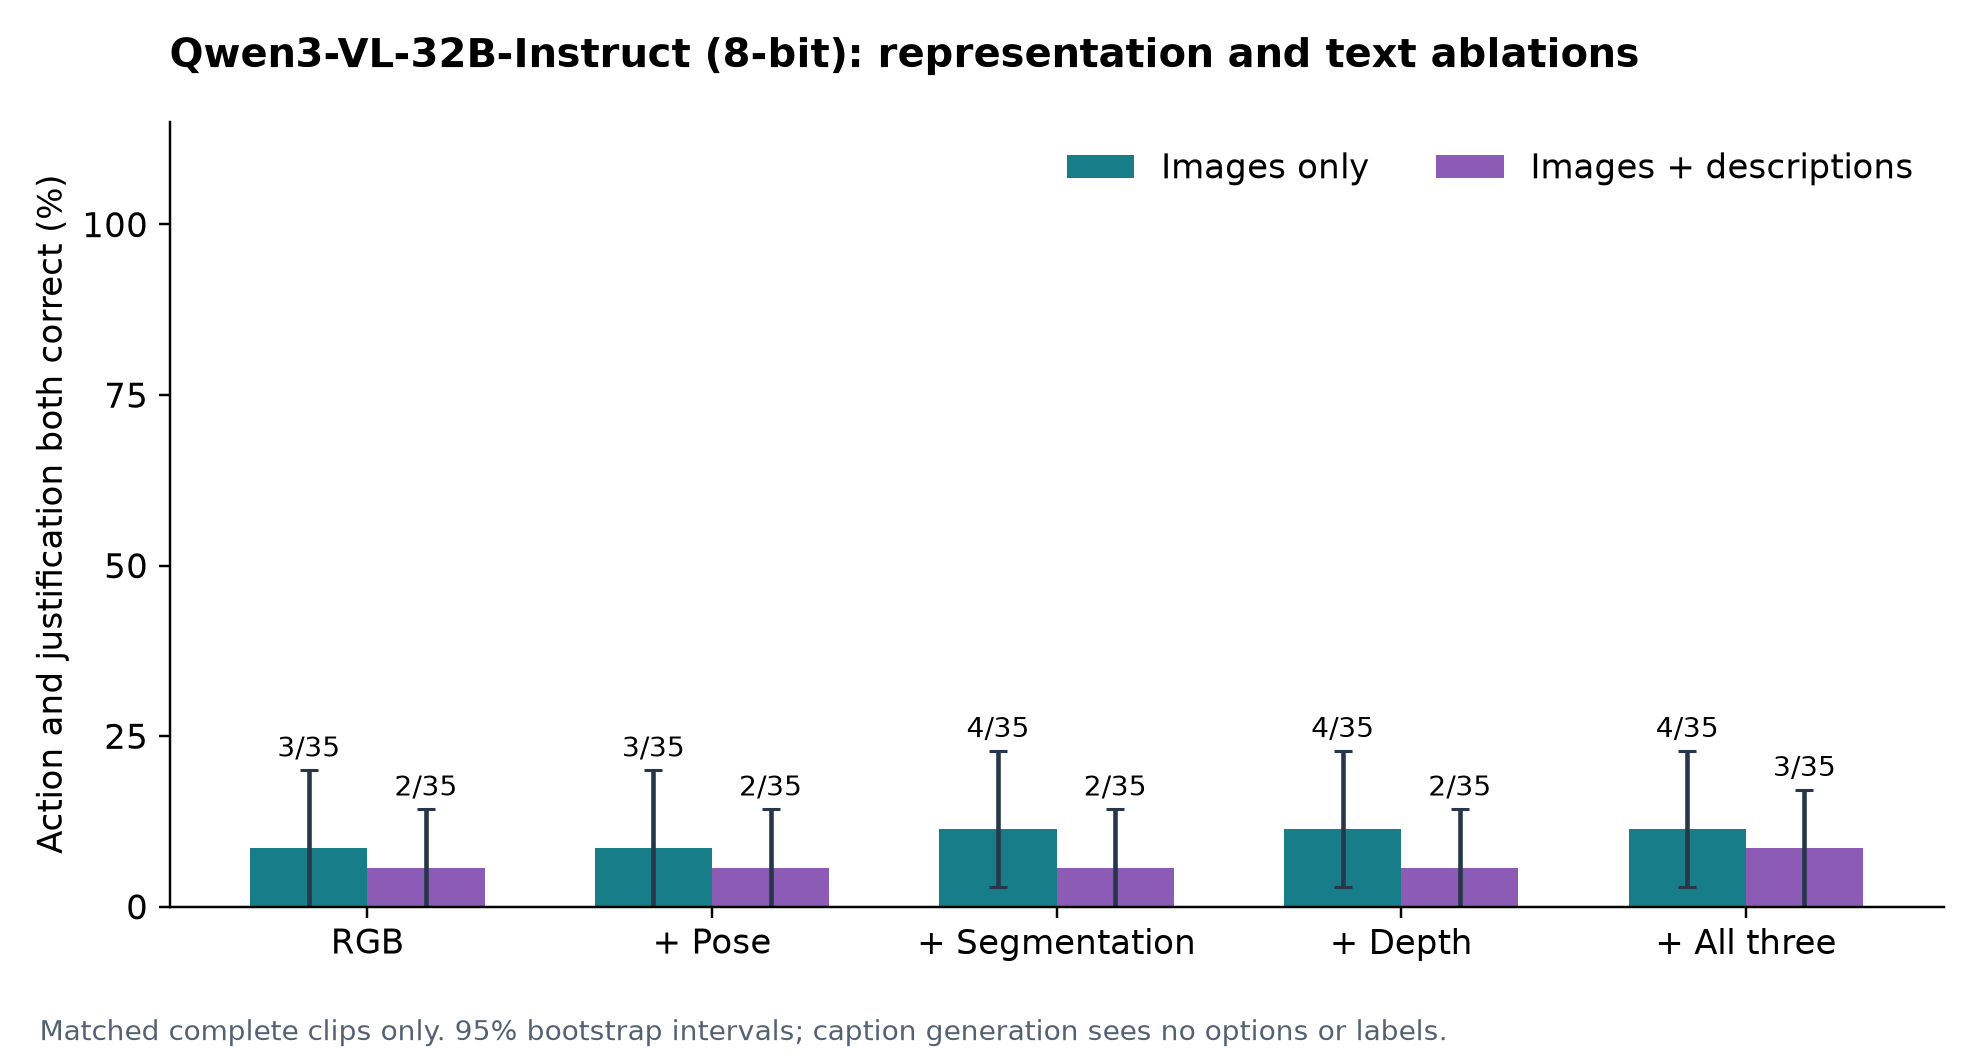
\includegraphics[width=\textwidth]{comparison.png}
\caption{Joint action and justification accuracy on the 35 fully evaluated source-disjoint clips (of 40 prepared). Bars compare images alone with images and attached descriptions. Error bars are empirical 95\% source-video bootstrap intervals, not a correction for multiple exploratory comparisons.}
\end{figure*}
\clearpage\onecolumn
\section*{AI usage and contribution record (draft)}
An OpenAI Codex agent inspected the assignment and proposal, designed the exploratory comparison and controls, implemented and debugged the download, extraction, inference, and reporting scripts, installed isolated environments, downloaded the public dataset and pretrained models, ran the computations, calculated statistics, and generated this provisional section, figure, and review gallery. AI assistance includes experiment design, code, execution, analysis summaries, and writing.

Frozen MediaPipe models generated body and hand landmark predictions. Frozen YOLOv8n-seg generated COCO-class instance masks; Depth Anything V2 Small generated uncalibrated relative monocular depth. A local community 8-bit Qwen3-VL-32B-Instruct checkpoint generated question-free RGB descriptions and experimental action/justification predictions. Processed-image descriptions summarize extractor outputs deterministically. A spawned agent configured with the requested gpt-5.6-sol override inspected actual images for a 15-example RGB baseline, a five-example representation pilot, and 15-condition diagnostics on four baseline failures. That pilot uses tools and accumulates context and is not a clean stateless API comparison. The agent could not independently inspect the served model identity. No model was trained.

The student selected idea 5 and requested these analyses. Personal review, final student interpretation, TA approval, and teammate contributions have not yet been recorded. Complete these details truthfully. The student must lead the final interpretation and disclose all AI assistance.
\section*{Reproducibility and limitations}
The dataset was downloaded at a pinned revision. The fixed sample, frame timestamps, model revisions and weight hashes, dependencies, prompts, option permutations, raw responses, captions, predictions, scores, and paired comparisons are saved in the accompanying project. Failed detections and invalid outputs remain in the denominator. The review gallery attaches descriptions to RGB, pose, segmentation, and depth grids for all 40 examples and allows review notes to be exported.

This is a custom subset experiment rather than a full-benchmark leaderboard reproduction. The representations are estimates derived from RGB, not independent physical measurements. Caption errors can influence decisions. Repeated-image controls match image slots and resolution but not description lengths. The new 32B prompt differs from the prior 8B pilot, preventing a clean model-size-only claim. Exploratory scoring uses EgoNormia labels, so these examples are not untouched test data for later model selection.
\section*{Sources}
\begin{itemize}
\item EgoNormia: \url{https://huggingface.co/datasets/open-social-world/EgoNormia}
\item Qwen checkpoint: \url{https://huggingface.co/mlx-community/Qwen3-VL-32B-Instruct-8bit}
\item Depth model: \url{https://huggingface.co/depth-anything/Depth-Anything-V2-Small-hf}
\item Segmentation: \url{https://docs.ultralytics.com/tasks/segment/}
\end{itemize}
\end{document}
